\section*{Постановка задачи}
Разработать консольную игру в парадигме объектно ориентированного
программирования на языке программирования \verb|Python|.

Ссылка на репозиторий с программами и отчёт написанный с помощью \LaTeX\@:
\url{https://github.com/andreymlv/tstu-computation-theory}
\addcontentsline{toc}{section}{Постановка задачи}

\section{Дизайн игры}

Центральным объектом в игре является игровое поле.
На игровом поле есть следующие объекты:
\begin{enumerate}
	\item База.
	\item Юниты.
	\item Ландшафт.
\end{enumerate}

Игровое поле можно разделить на ячейки, которые будут хранить в себе игровые объекты.
На текущий момент ячейка хранит в себе свои координаты в игровом поле, объекты базы,
юнита, курсора и ландшафта.

Игровой курсор представляет собой интерфейсом взаимодействия игры и игрока.

Управление курсора возможно с помощью клавиатуры.

Чтобы играть необходим терминал, который поддерживает \verb|ASCII| коды.
Они необходимы для того, чтобы были видны цвета.

\begin{figure}[H]
	\begin{center}
		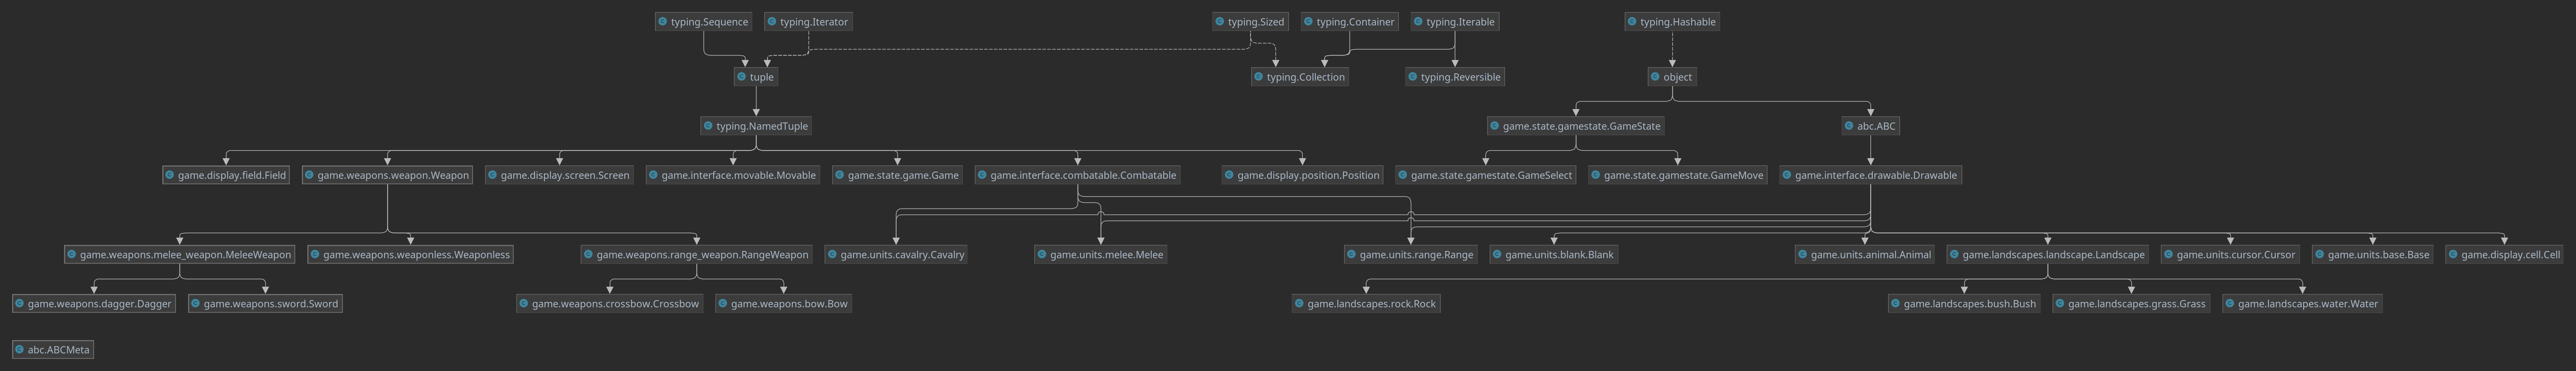
\includegraphics[width=\textwidth]{game.png}
		\caption{Диаграмма классов}
	\end{center}
\end{figure}

\section{Детали реализации}

Как можно видеть из диаграммы классов, большинство объектов унаследованы либо от
\verb|NamedTuple| или декорируются с помощью \verb|dataclass|ов.

По ходу написания реализации проект был полностью переписан, из-за изначально неверных
архитектурных решений.

В итоге использовались следующие шаблоны проектирования и подходы реализации:

\begin{itemize}
  \item Шаблон состояние. Выделили состояние ``игра'', где управление клавиатурой 
    переводит игру в новое состояние. Каждое новое состояние игры является новым объектом.
  \item Неизменяемые объекты. 
    Поля объектов являются неизменяемыми во время исполнения.
  \item Декларативное программирование. 
    В итоге наша реализация является композицией функций
    (считаем, что создание нового объекта тоже является функцией).
  \item Предпочитаем композицию вместо наследования.
  \item Не используем \verb|None| объекты. Таким образом избегаем \verb|NullPointerException|.
  \item Используем типизацию.
  \item Не используем статические методы.
  \item Не используем глобальные переменные.
  \item Не используем \verb|mixin|ы. Так как в \verb|Python| можно использовать абстрактные классы или интерфейсы (класс \verb|ABC|).
\end{itemize}

\begin{figure}[H]
	\begin{center}
		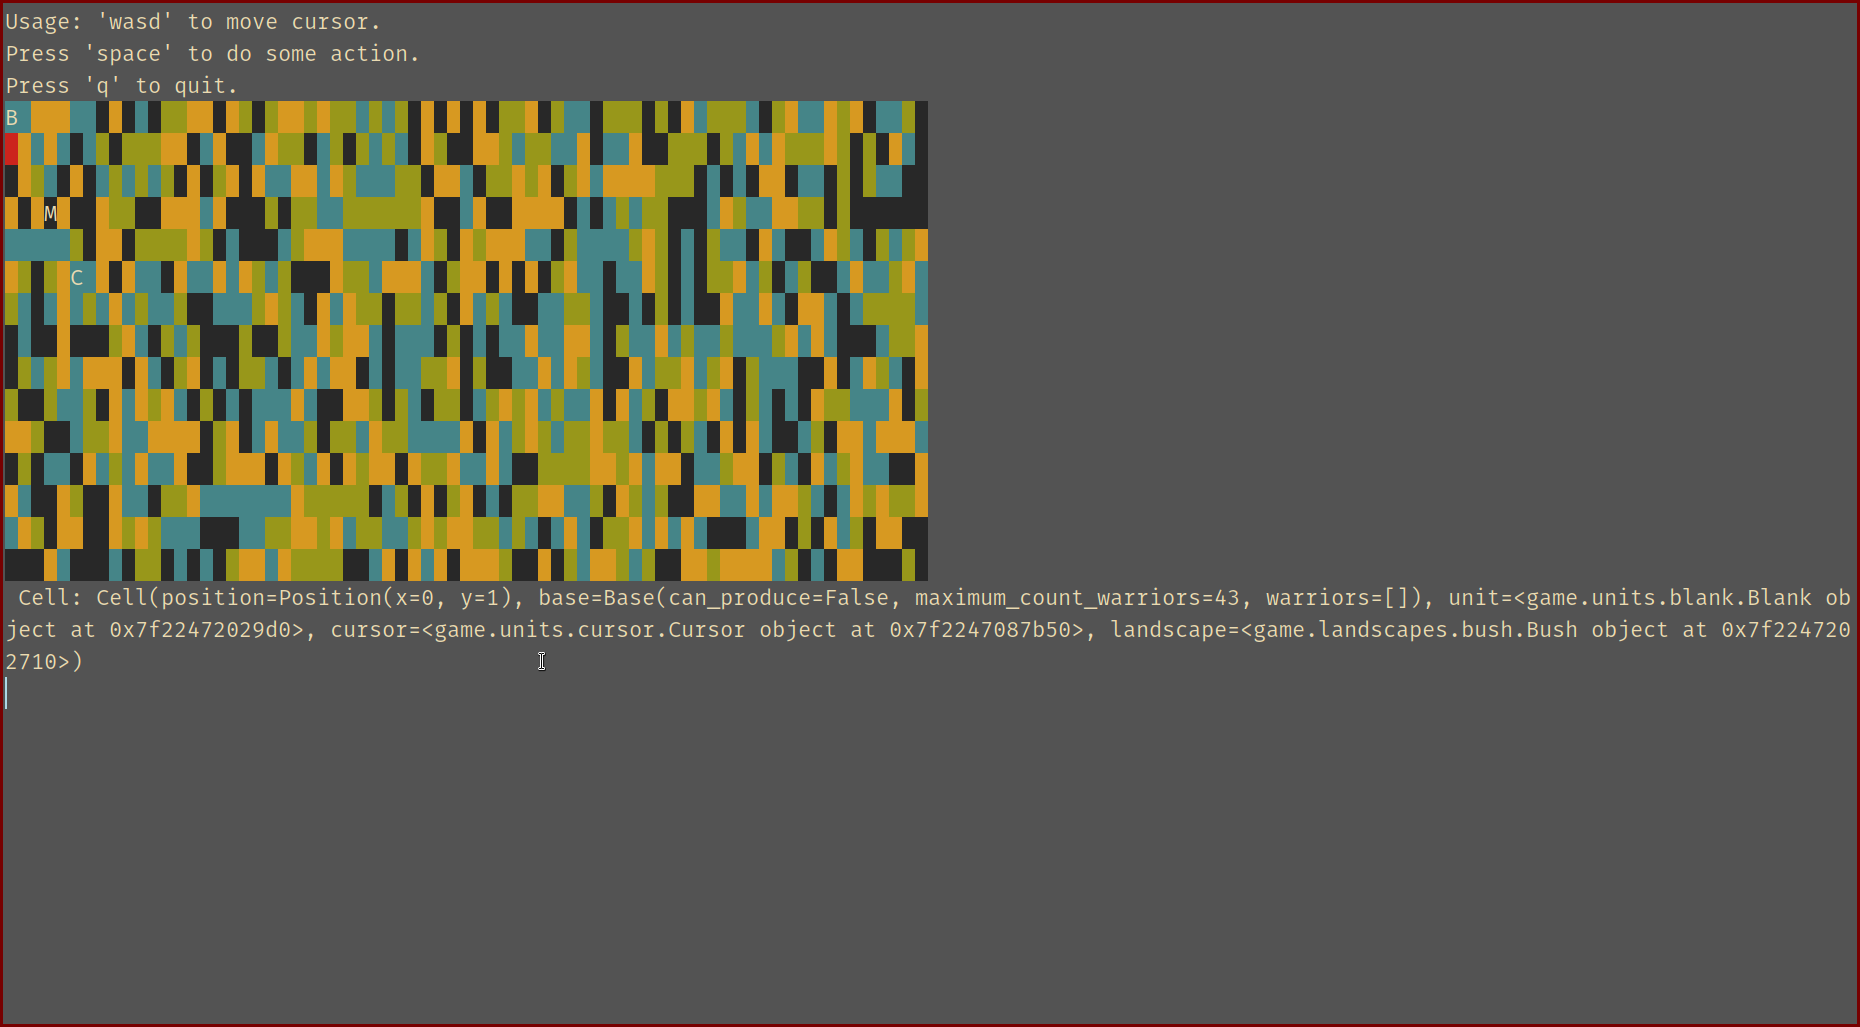
\includegraphics[width=\textwidth]{start-game.png}
		\caption{Запущенная игра}
	\end{center}
\end{figure}

\begin{figure}[H]
	\begin{center}
		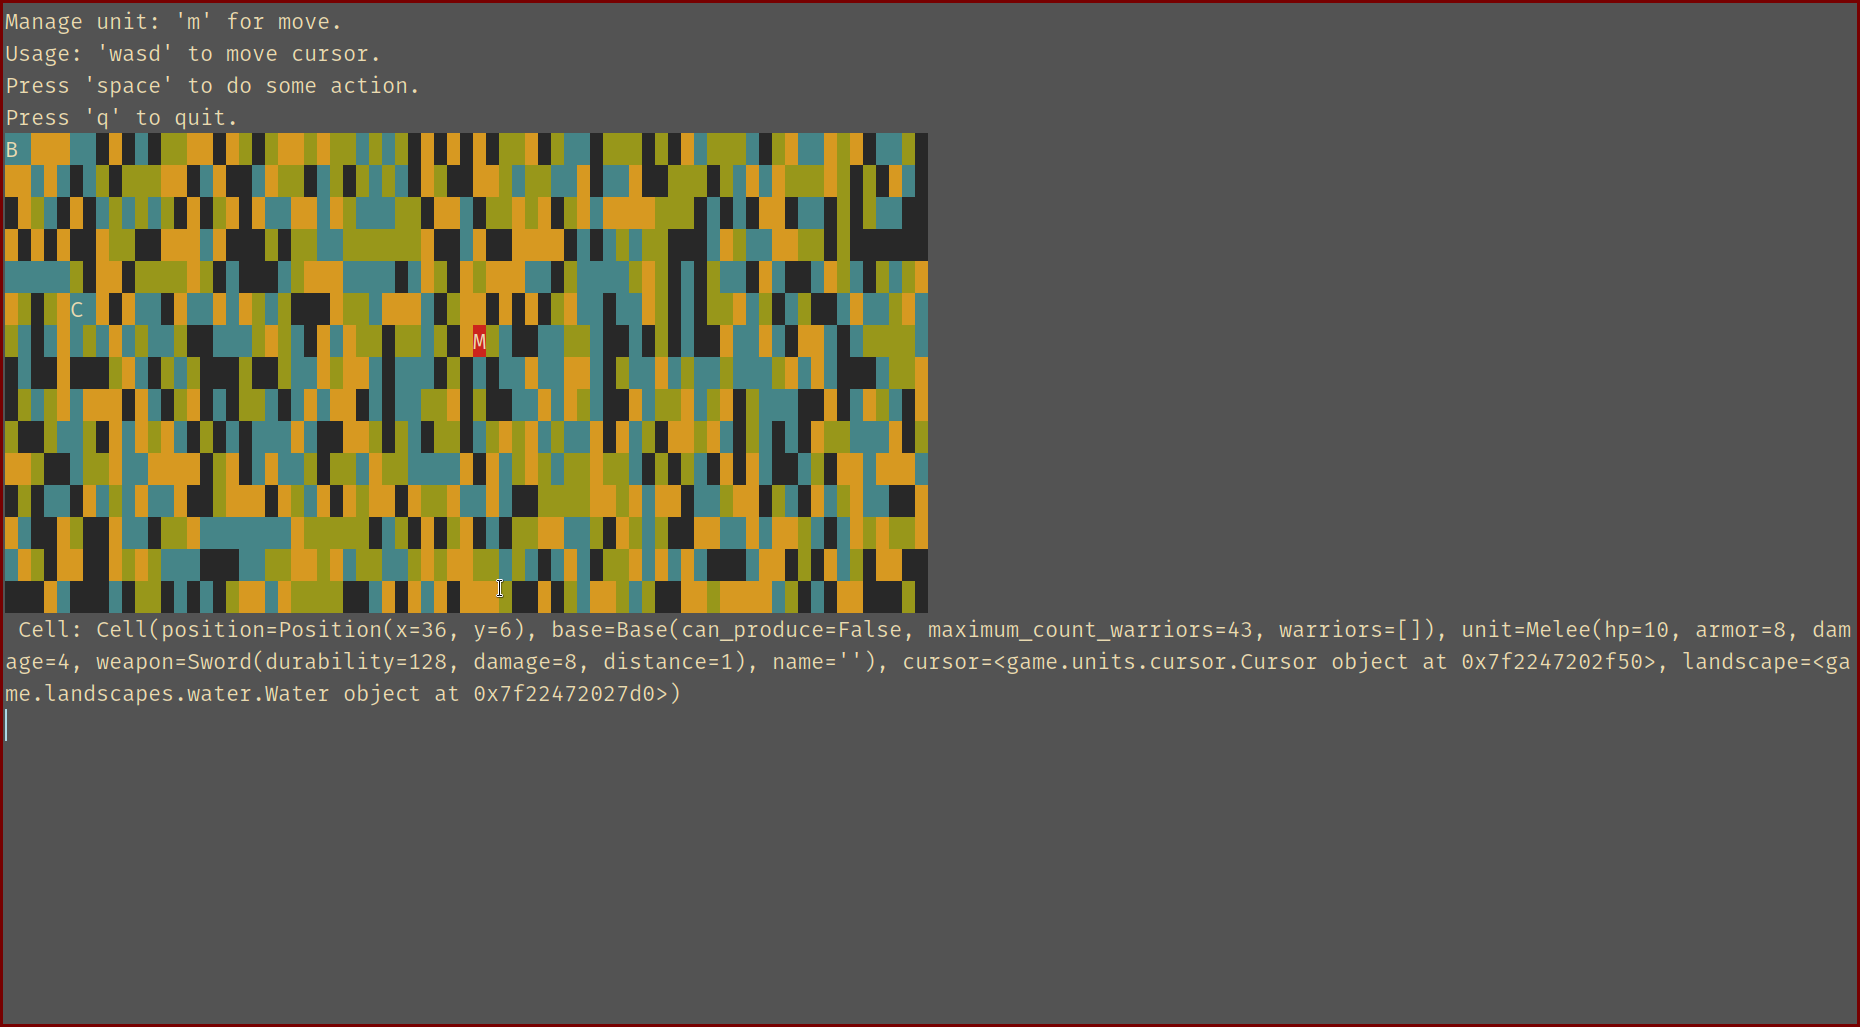
\includegraphics[width=\textwidth]{unit-menu.png}
		\caption{Запущенная игра}
	\end{center}
\end{figure}

\begin{figure}[H]
	\begin{center}
		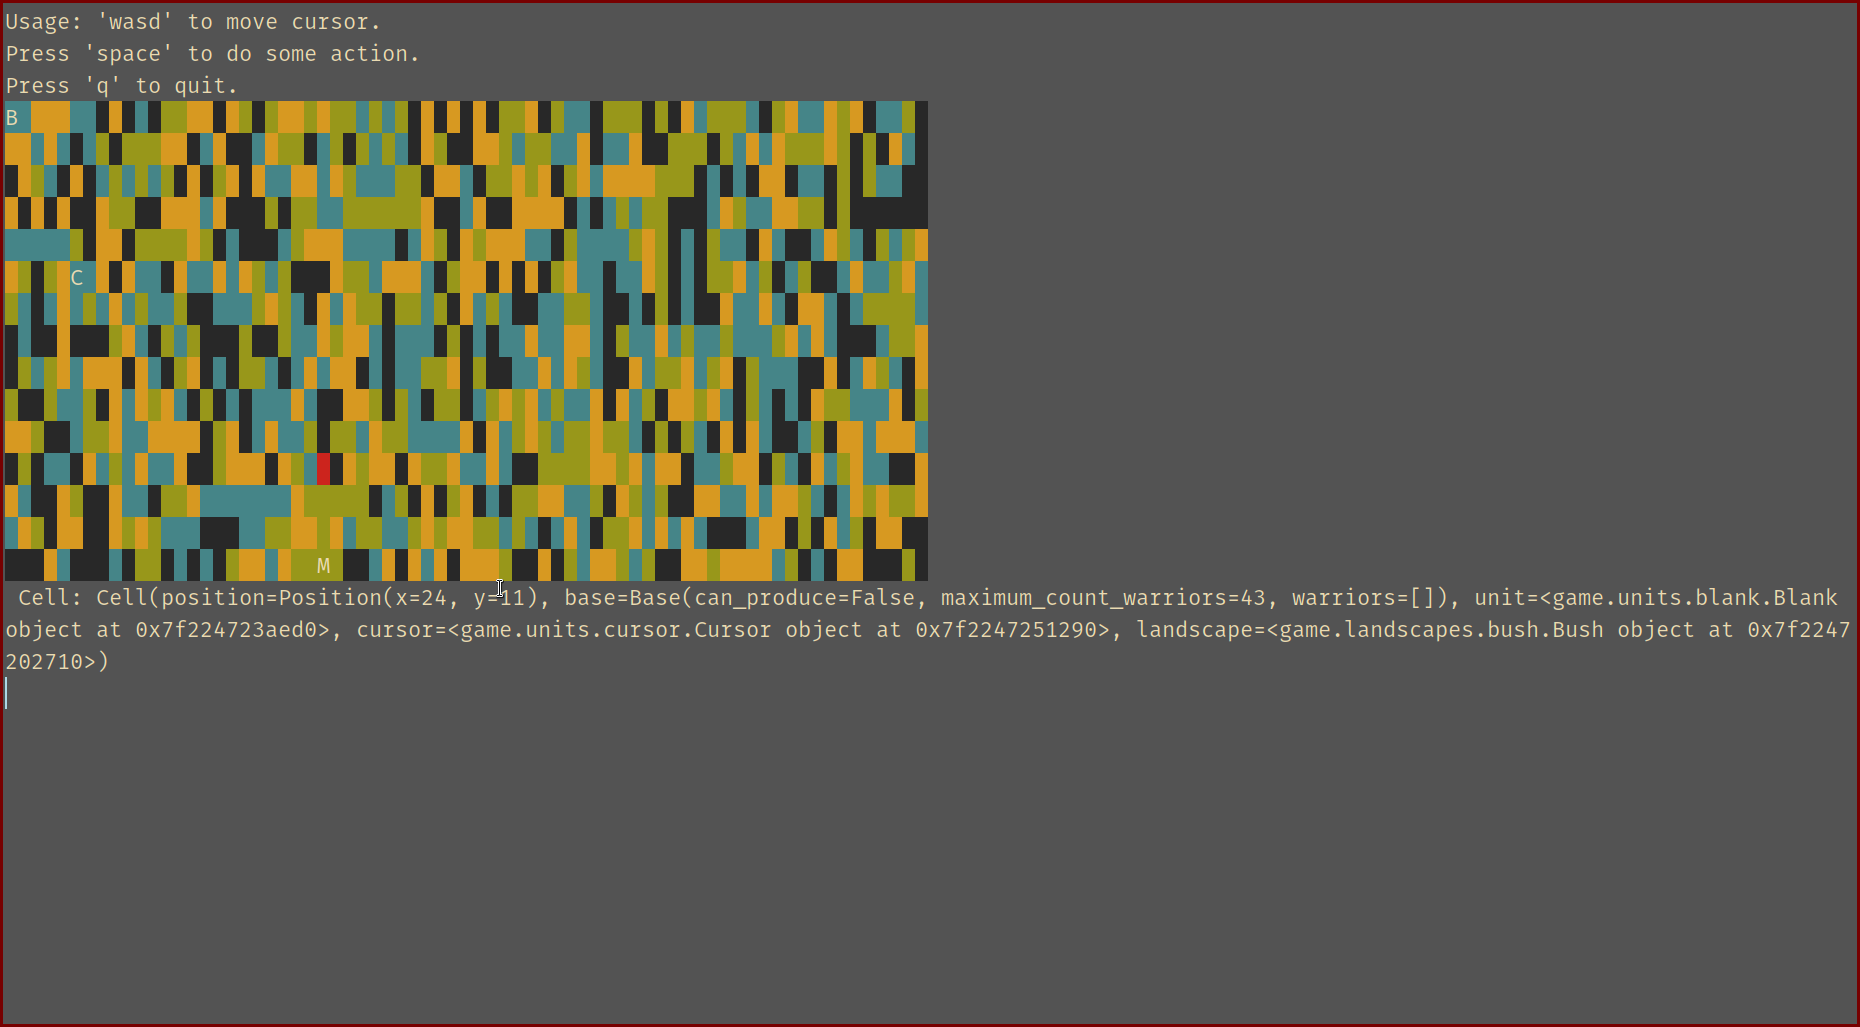
\includegraphics[width=\textwidth]{after-unit-move.png}
		\caption{Запущенная игра}
	\end{center}
\end{figure}

Главный скрипт, который инициализирует и запускает цикл игры выглядит примитивно.
Сначала инициализируем игровое поле. Заполняем клетки игры объектами.
Запускаем цикл игры: очищаем экран, печатаем текущее состояние игры, 
переводим игру в новое состояние (действия, которые независимы от ввода игрока), 
и затем снова переводим игру в новое состояние, где мы читаем ввод игрока.

\begin{code}
	\inputminted[breaklines=true, xleftmargin=1em, linenos, frame=single, framesep=10pt, fontsize=\footnotesize, firstline=1, lastline=120]{python}{../src/main.py}
	\caption{main.py --- главный скрипт игры}
\end{code}

\section*{Заключение}
Реализовали консольную игру, используя принципы объектно ориентированного программирования.
\addcontentsline{toc}{section}{Заключение}
